KOMMENTAR ZUM GESAMTEN DOKUMENT
%- Du musst in deinen Beschreibungen auch nicht davon ausgehen, dass du die App jemandem erklärst, der noch nie eine App verwendet hat. So knapp  und übersichtlich wie möglich ist dein Ziel. Viel Text bedeutet, unsere App ist zu kompliziert, dass wir jede Menge Text zum erklären brauchen. 
%-achte drauf, dass du bei Beschreibung, Elemente und Verwendung nichts doppelt schreibst... das ist ein paar mal zu 80% dasselbe
%-das Wort "Tippen" so gut wie möglich vermeiden

%- ich muss sagen, dass es sehr anstrengend ist den Text zu lesen, dabei sollte es kurz und knackig und informativ sein. Ich fühl mich eher, wie wenn ich grade 100 mal dasselbe gelesen habe und hatte gegen Ende keine Lust mehr bzw. war mir schon sicher zu wissen, was drin steht. 

\section{Benutzerschnittstelle}
\begin{wrapfigure} {L}{0.35\textwidth}
\caption{Erste Startansicht}
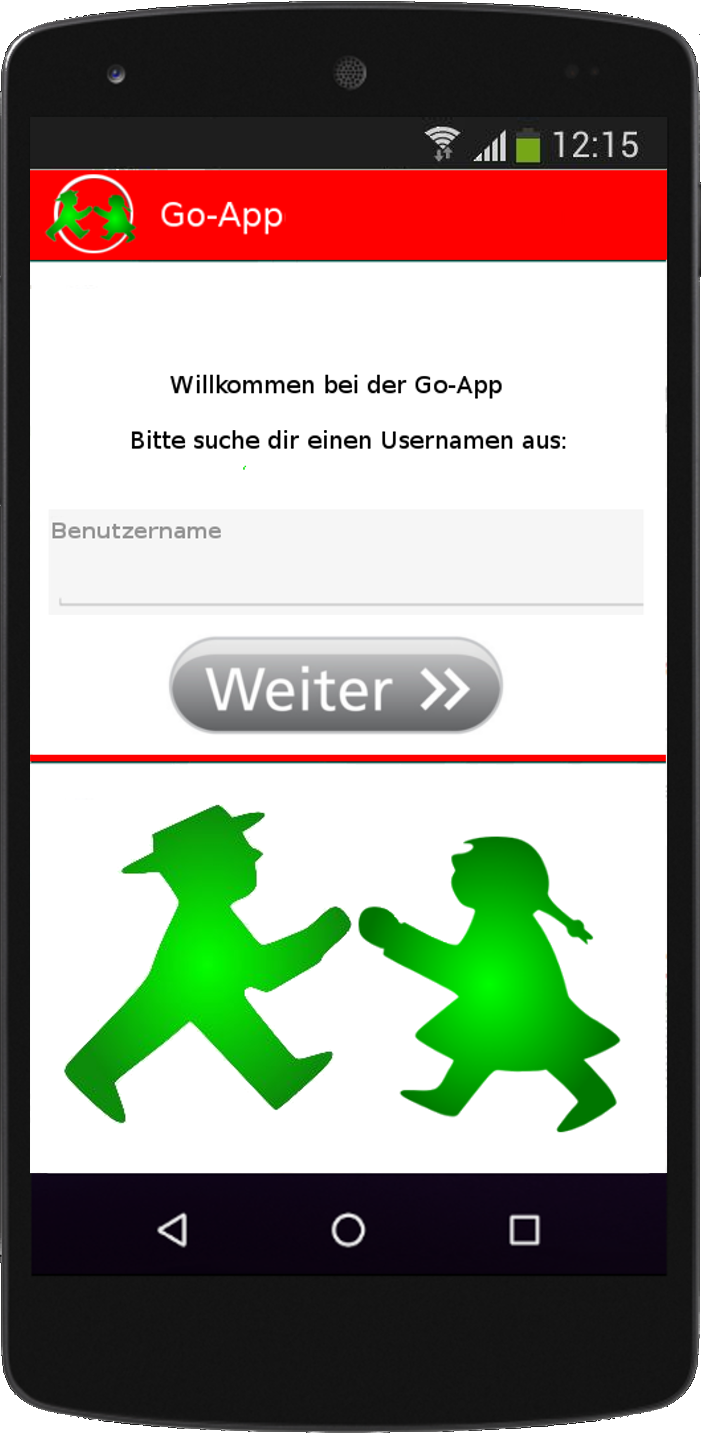
\includegraphics[scale = 0.2]{resources/images/handy/startansicht.png}
\end{wrapfigure}


\textbf{Beschreibung:}\\
Erste Startansicht der Go-App, Aufforderung an den neuen Benutzer einen Benutzernamen zu wählen.\\
\textbf{Elemente:}\\
Textfeld "Benutzername" zum Einfügen des Benutzernamens.\\
"Weiter"-Button um diesen zu bestätigen.\\
\textbf{Verwendung:}\\
Durch einmaliges Tippen auf das Textfeld "Benutzername" wird die Bildschirmtastatur aktiviert und der Benutzer kann seinen gewählten Benutzernamen eingeben.\\
Durch einmaliges Tippen auf den "Weiter"-Button wird dieser Benutzername bestätigt und der Benutzer wird zur Gruppenübersicht weitergeleitet.

\newpage

\begin{wrapfigure} {L}{0.35\textwidth}
	\caption{Gruppenübersicht}
%\begin{center}
	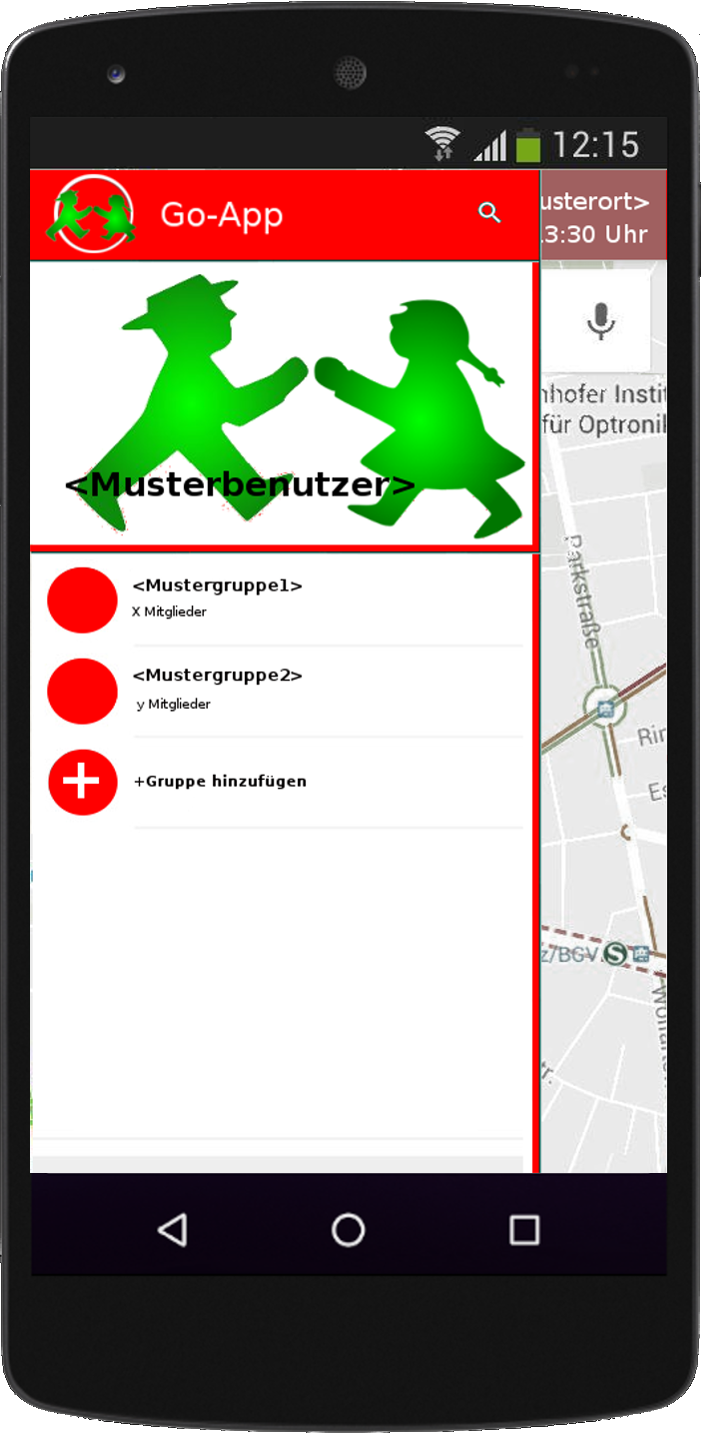
\includegraphics[scale = 0.2]{resources/images/handy/gruppenuebersicht.png}
%\end{center}
\end{wrapfigure}

\textbf{Beschreibung:}\\
Übersicht über die Gruppen, in denen der Benutzer Mitglied ist. Wenn dieser das erste Mal zu der angegebenen Ansicht gelangt, ist er noch kein Mitglied einer Gruppe und deshalb werden ihm auch noch keine angezeigt.\\
\textbf{Elemente:}\\
Benutzernahme zur Orientierung, mit welchem Namen der Benutzer registriert ist.\\
Gruppennamen zur Übersicht über die Gruppen, in denen der Benutzer Mitglied ist.\\
"Gruppe hinzufügen"-Button um eine neue Gruppe hinzuzufügen.\\
\textbf{Verwendung:}\\
WK(Wunschkriterium): Durch einmaliges Tippen auf den Benutzernamen wird der Benutzer weitergeleitet zur Option Benutzername ändern.\\
Durch einmaliges Tippen auf einen Gruppennamen wird der Benutzer weitergeleitet zur Kartenansicht der Gruppe.\\
Durch langes Tippen auf einen Gruppennamen kann der Benutzer "aus der Gruppe austreten" wählen bzw. der GA (Gruppenadministrator) "Gruppe löschen".\\
Durch einmaliges Tippen auf den "Gruppe hinzufügen"-Button wird der Benutzer weitergeleitet zur Option "Gruppe hinzufügen".\\
Durch Streichen nach oben oder unten kann der Benutzer durch die Gruppen scrollen, wenn es mehr sind als auf den Bildschirm passen.\\
Durch Streichen von rechts nach links kann man die Gruppenansicht weg schieben und gelangt zu der zuletzt verwendeten Karte.
\newpage

%KOMMENTAR
%-ich würde die Wörter Button soweit als möglich vermeiden und einfach: über "Gruppe hinzufügen" kann eine neue Gruppe erstellt werden
%-auch hier würde ich Tippen so gut wie möglich wieder weglassen, nur wenn es wirklich wichtig ist. Und ich glaube langes Tippen gibt es nicht... zumindest hört es sich komisch 

\begin{wrapfigure} {L}{0.35\textwidth}
	\caption{Gruppe erstellen}
%\begin{center}
	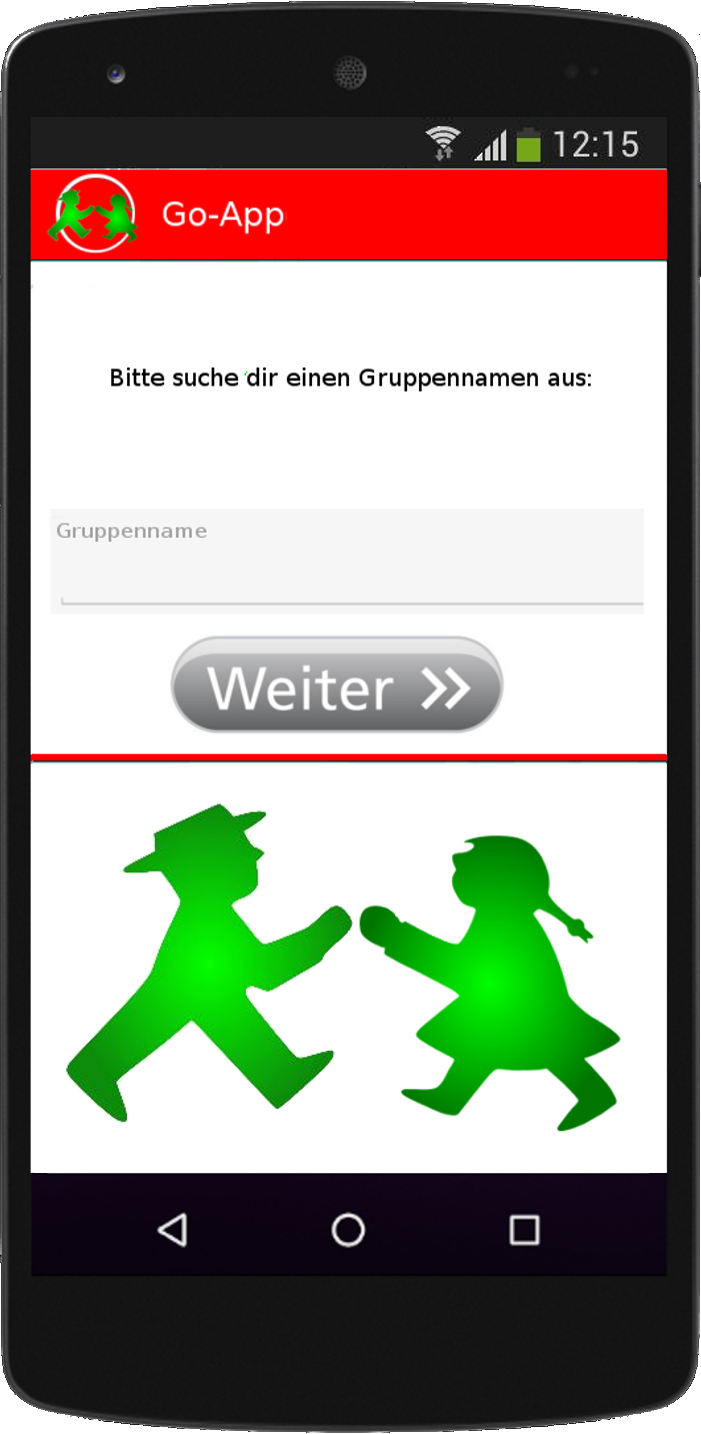
\includegraphics[scale =0.2]{resources/images/handy/gruppe_erstellen.png}
%\end{center}
\end{wrapfigure}

\textbf{Beschreibung:}\\
Option Gruppe hinzufügen, Aufforderung an den Benutzer sich einen Gruppennamen zu wählen.\\
\textbf{Elemente:}\\
Textfeld "Gruppenname" zum Einfügen des Gruppennamens.\\
"Weiter"-Button um diesen zu bestätigen.\\
\textbf{Verwendung:}\\
Durch einmaliges Tippen auf das Textfeld "Gruppenname" wird die Bildschirmtastatur aktiviert und der Benutzer kann seinen gewählten Gruppennamen eingeben.\\
Durch einmaliges Tippen auf den "Weiter"-Button wird dieser Gruppenname überprüft. Ist dieser noch nicht vergeben, wird er bestätigt und der Benutzer wird weitergeleitet zur Gruppenübersicht. Gibt es bereits eine Gruppe die den gewählten Namen trägt, wird der Benutzer aufgefordert einen anderen Gruppennamen auszuwählen.
\newpage

\begin{wrapfigure} {L}{0.35\textwidth}
	\caption{Karten-Ansicht der Gruppe (leer)}
%\begin{center}
	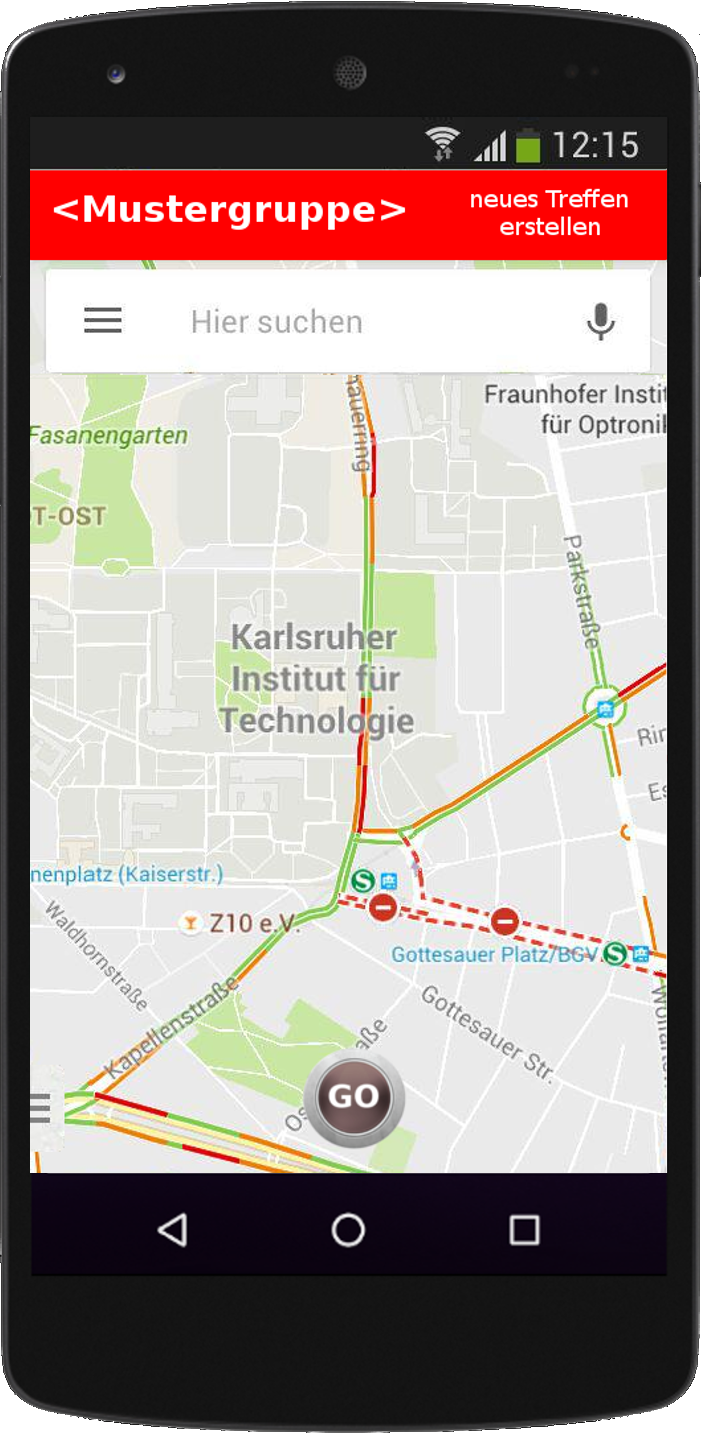
\includegraphics[scale =0.2]{resources/images/handy/map_leer_admin.png}
%\end{center}
\end{wrapfigure}

\textbf{Beschreibung:}\\
Kartenansicht der Gruppe. Wenn der GA(Gruppenadministrator) das erste Mal zu dieser Ansicht gelangt, hat er noch keine Treffen erstellt und somit wird ihm auch noch eine leere Karte angezeigt. Ebenso wenn er kein aktuelles Treffen erstellt hat, wird allen GM(Gruppenmitgliedern) eine leere Karte angezeigt.\\
\textbf{Elemente:}\\
"Gruppenname"-Button um zu den Gruppendetails zu gelangen.\\
"neues Treffen erstellen"-Button bei der Ansicht des GA um ein neues Treffen zu erstellen, bzw. "kein aktuelles Treffen"-Anzeige bei der Ansicht aller GM ohne besondere Rechte.\\
"Hier suchen"-Textfeld um einen Ort auf der Karte zu suchen.\\
Handle links unten in der Ecke um die Gruppenansicht wieder herauszuziehen.\\
"Go"-Button ausgegraut bei Inaktivität.\\
\textbf{Verwendung:}\\
Durch einmaliges Tippen auf den "Gruppenname"-Button wird das GM weiter geleitet zu der Ansicht "Gruppendetails".\\
Durch einmaliges Tippen auf den "neues Treffen erstellen"-Button wird der GA weiter geleitet zu der Option "Treffen erstellen", für alle anderen GM ist diese "kein aktuelles Treffen"-Anzeige lediglich informativ.\\
Durch einmaliges Tippen auf das Textfeld "Hier suchen" wird die Bildschirmtastatur aktiviert und das GM kann seinen gewählten Ort eingeben.\\
Durch Streichen von links nach rechts über den Handle-Button kann das GM die Gruppenansicht wieder herausziehen.
\newpage

%KOMMENTAR
%-du erklärst teilweise bei Elemente schon, was diese machen und dann bei Verwendung nochmal: "neues Treffen erstellen"-Button bei der Ansicht des GA um ein neues Treffen zu erstellen"
%Durch einmaliges Tippen auf den "neues Treffen erstellen"-Button wird der GA weiter geleitet zu der Option "Treffen erstellen"
\begin{wrapfigure} {L}{0.35\textwidth}
	\caption{Übersicht über die Gruppenmitglieder}
%\begin{center}
	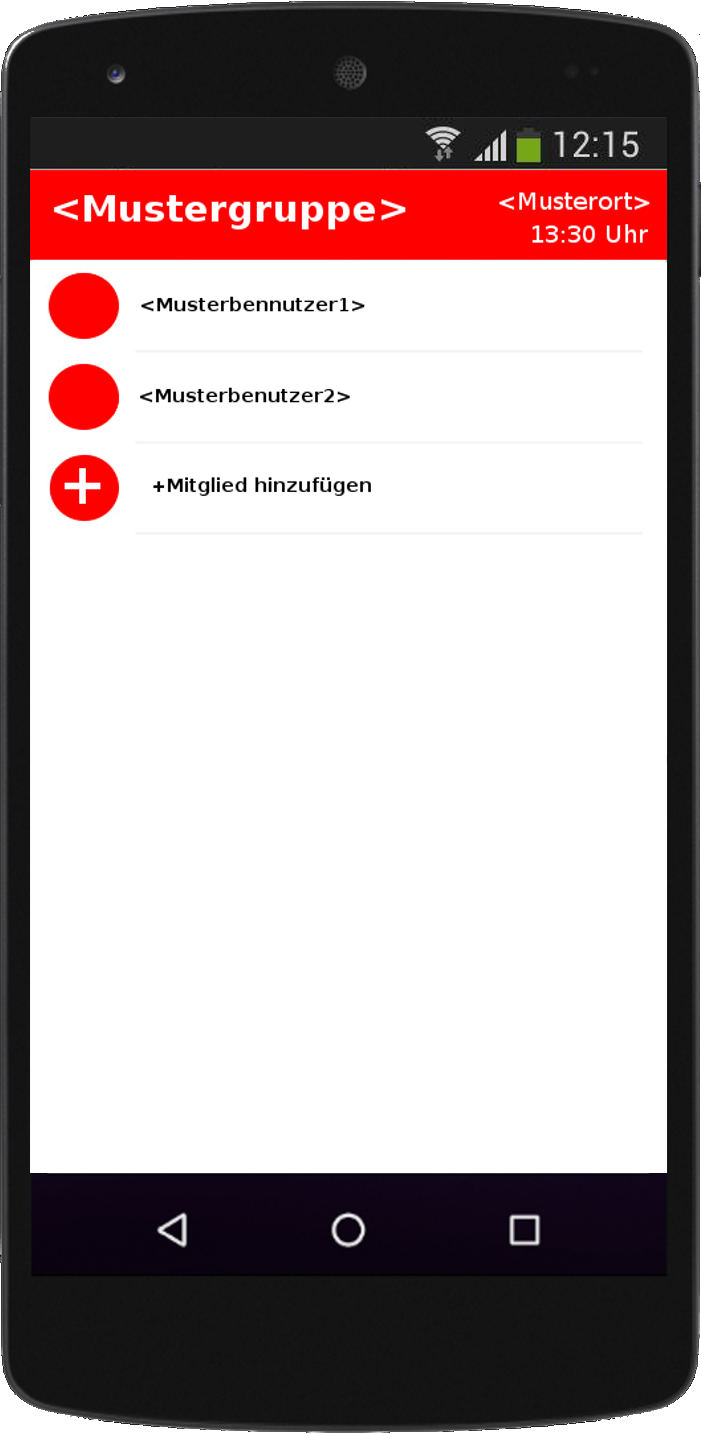
\includegraphics[scale =0.2]{resources/images/handy/gruppendetails_admin.png}
%\end{center}
\end{wrapfigure}

\textbf{Beschreibung:}\\
Übersicht über die GMer. Wenn der GA das erste Mal zu dieser Ansicht gelangt, ist außer ihm noch kein weiteres Mitglied in dieser Gruppe.\\
\textbf{Elemente:}\\
"Gruppenname"-Button zur Übersicht, in welcher Gruppe das GM aktiv ist und um zurück zur Karten-Ansicht der Gruppe zu gelangen.\\
"neues Treffen erstellen"-Button oder "Uhrzeit"-Button bei der Ansicht des GA um ein neues Treffen zu erstellen, bzw. "kein aktuelles Treffen"-Anzeige oder "Uhrzeit"-Anzeige bei der Ansicht aller GMG ohne besondere Rechte.\\
Mitgliedernamen zur Übersicht über die Mitglieder der Gruppe.\\
"Mitglied hinzufügen"-Button um ein neues GM einzuladen aus Ansicht des GA.\\
\textbf{Verwendung:}\\
Durch einmaliges Tippen auf den "Gruppenname"-Button wird der Gruppenadministrator zurück geleitet zu der Kartenansicht der Gruppe.\\
"neues Treffen erstellen"-Button bzw. Uhrzeit-Button hat die selbe Funktion wie in der Kartenansicht der Gruppe.\\
Durch einmaliges Tippen auf den "Mitglied hinzufügen"-Button öffnet sich das Fenster "Link versenden".
\newpage

%KOMMENTAR
%-in welcher Gruppe man gerade aktiv ist, sieht man doch schon am Gruppennamen, da muss man doch nicht erst noch drauf gehen und nachschauen (oder was sieht man da was man nicht schon am Gruppennamen sieht)

\begin{wrapfigure} {L}{0.35\textwidth}
	\caption{Link versenden}
%\begin{center}
	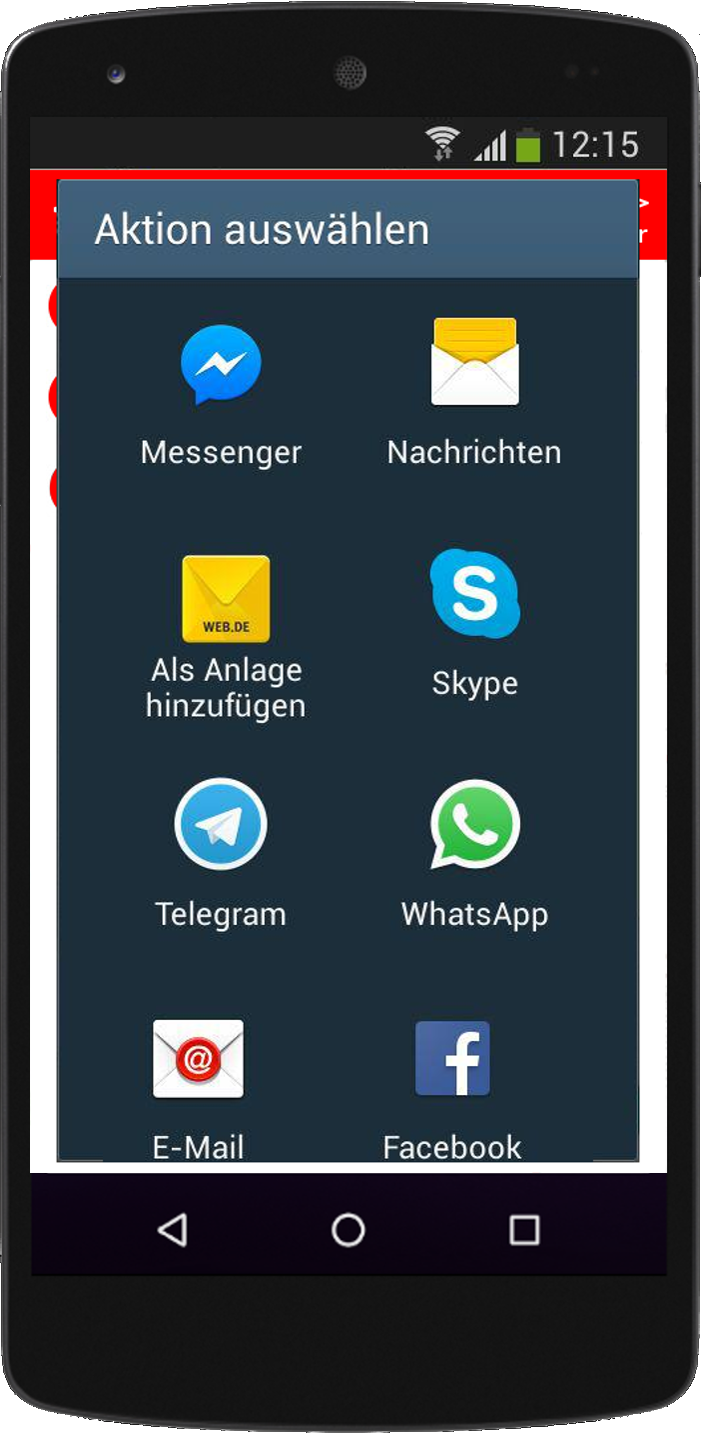
\includegraphics[scale =0.2]{resources/images/handy/link_versenden.png}
%\end{center}
\end{wrapfigure}

\textbf{Beschreibung:}\\
Übersicht über verschiedene Kommunikationswege, die verwendet werden können um andere GM in die Gruppe einzuladen.\\
\textbf{Elemente:}\\
Auswahlmöglichkeiten der Kommunikationswegen, die der GA auf seinem Android-Gerät installiert hat.\\
\textbf{Verwendung:}\\
Durch einmaliges Tippen auf einen der Buttons wird der GA weitergeleitet zu der ausgewählten Applikation über die er dann den neu generierten Gruppen-Einladungs-Link versenden kann.
\newpage

\begin{wrapfigure} {L}{0.35\textwidth}
	\caption{Treffen erstellen}
%\begin{center}
	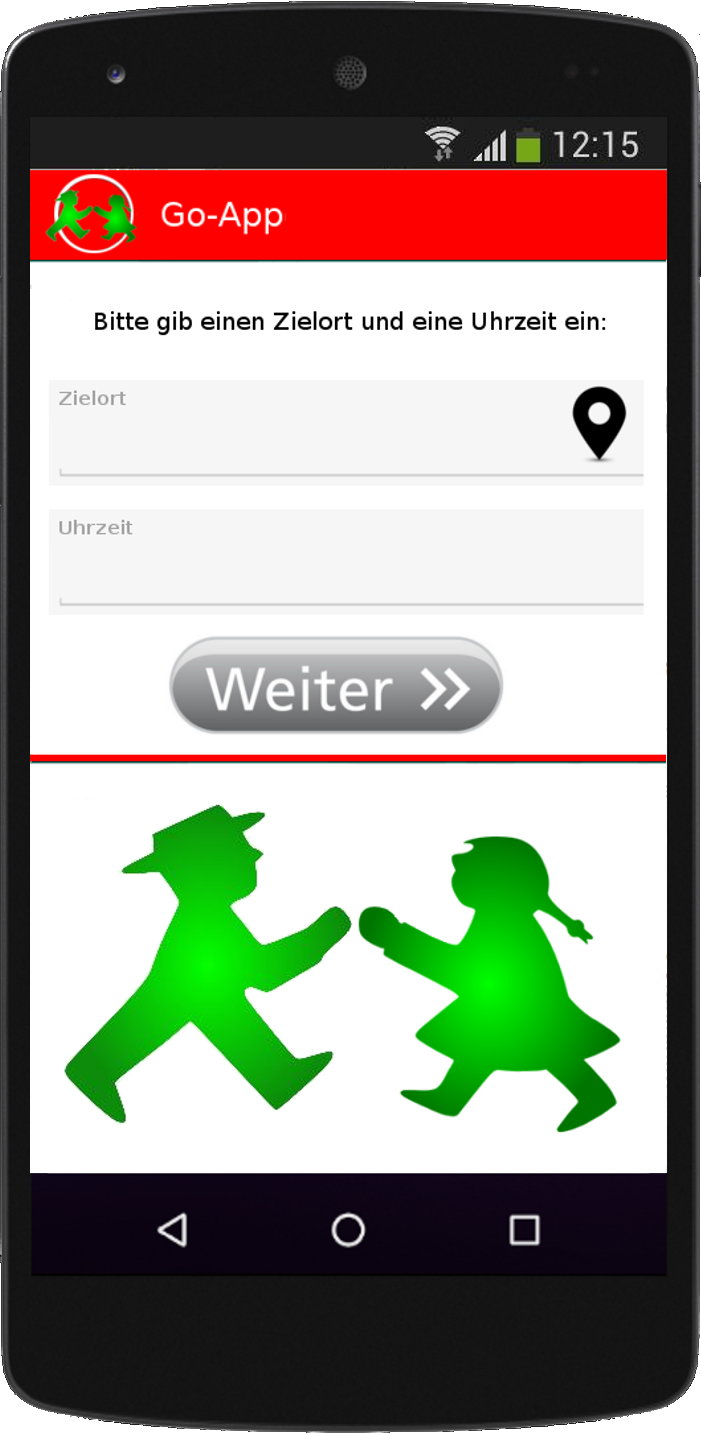
\includegraphics[scale =0.2]{resources/images/handy/treffpunkt_erstellen.png}
%\end{center}
\end{wrapfigure}

\textbf{Beschreibung:}\\
Option zum Erstellen eines neuen Treffens, Aufforderung an den Gruppenadministrator einen Zielort und eine Uhrzeit zu wählen.\\
\textbf{Elemente:}\\
Textfeld "Zielort" zum Einfügen des Zielortes.\\
Karten-Symbol-Button zum Auswählen des Zielortes per Karte.\\
Textfeld "Uhrzeit" zum Einfügen der Uhrzeit.\\
"Weiter"-Button um diese zu bestätigen.\\
\textbf{Verwendung:}\\
Durch einmaliges Tippen auf das Textfeld "Zielort" wird die Bildschirmtastatur aktiviert und der GA kann seinen gewählten Zielort eingeben.\\
Alternativ: durch einmaliges Tippen auf den Karten-Symbol-Button wird der GA weitergeleitet zu der Kartenansicht und kann dort durch einmaliges Tippen auf einen Ort diesen als Zielort eingeben.\\
Durch einmaliges Tippen auf das Textfeld "Uhrzeit" wird die Bildschirmtastatur aktiviert und der GA kann seine gewählte Zielzeit eingeben.\\
Durch einmaliges Tippen auf den "Weiter"-Button werden dieser Zielort und diese Uhrzeit überprüft. Sind die Eingaben zulässig, werden diese bestätigt und der Gruppenadministrator wird weitergeleitet zu der Kartenansicht der Gruppe. Sind Zielort und Uhrzeit nicht gültig, wird der GA aufgefordert einen anderen Ort, bzw. eine andere Zeit auszuwählen
\newpage

%KOMMENTAR
%- siehe Anfangskommentare oder die von den anderen 


\begin{wrapfigure} {L}{0.35\textwidth}
	\caption{Karten-Ansicht der Gruppe}
%\begin{center}
	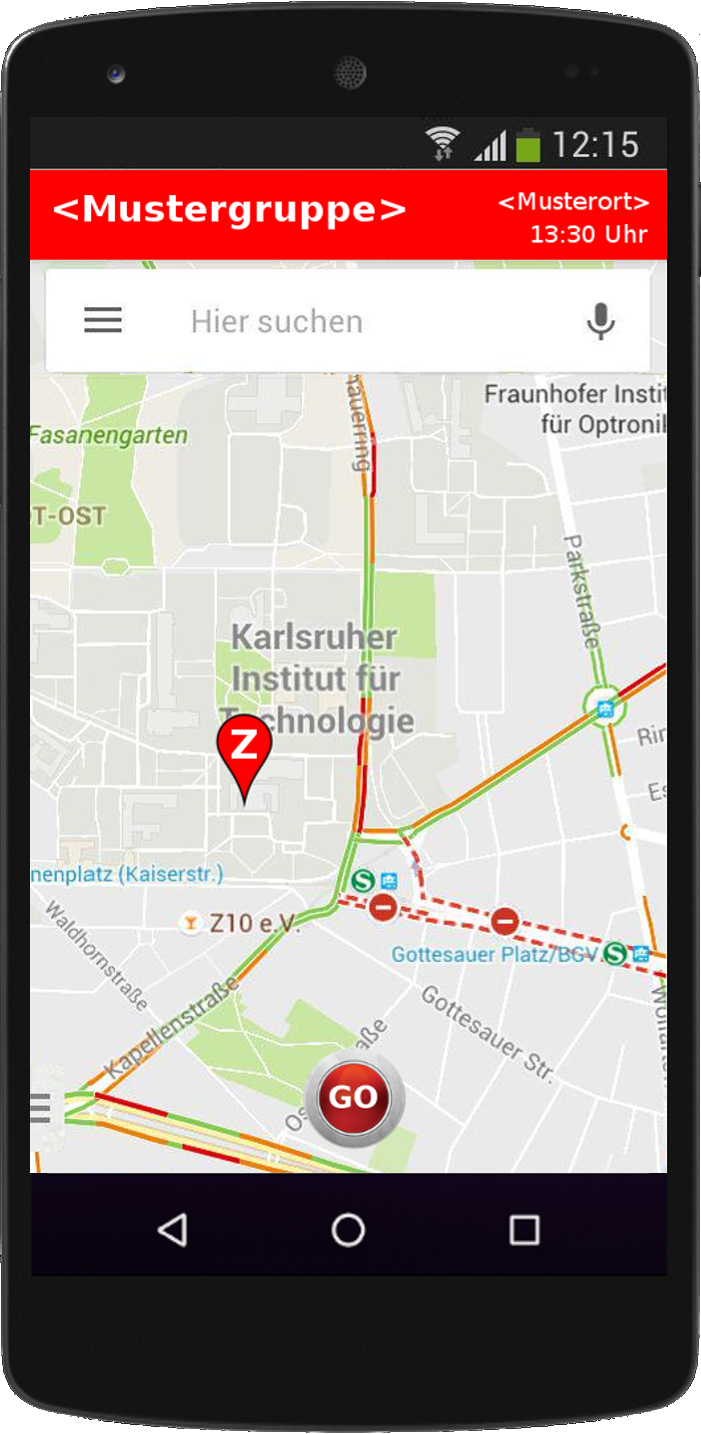
\includegraphics[scale =0.2]{resources/images/handy/map.png}
%\end{center}
\end{wrapfigure}

\textbf{Beschreibung:}\\
Kartenansicht der Gruppe mit festgelegtem Treffpunkt. Allen GMern wird in dieser Ansicht nicht nur die Karte angezeigt, sondern auch der Zielort und die Uhrzeit des nächsten festgelegten Treffpunktes, außerdem noch auf der Karte der Zielort durch eine Stecknadel beschriftet mit "Z".\\
\textbf{Elemente:}\\
"Gruppenname"-Button um zu den Gruppendetails zu gelangen.\\
"Zielort - Uhrzeit"-Ansicht zur Orientierung wann und wo das nächste Treffen statt findet, bzw. "Zielort - Uhrzeit"-Button bei der Ansicht des GA um ein neues Treffen zu erstellen.\\
"Hier suchen"-Textfeld um einen Ort auf der Karte zu suchen.\\
Handle links unten in der Ecke um die Gruppenansicht wieder herauszuziehen.\\
Aktivierter "Go"-Button um anzuzeigen, wann man los geht.
\textbf{Verwendung:}\\
Durch einmaliges Tippen auf den "Gruppenname"-Button wird das GM weiter geleitet zu der Ansicht "Gruppendeteils".\\
Durch einmaliges Tippen auf den "Zielort - Uhrzeit"-Button wird der GA weiter geleitet zu der Option "Treffen erstellen".\\
Durch einmaliges Tippen auf das Textfeld "Hier suchen" wird die Bildschirmtastatur aktiviert und das GM kann seinen gewählten Ort eingeben.\\
Durch Streichen von links nach rechts über den Handle-Button kann das GM die Gruppenansicht wieder herausziehen.\\
Durch einmaliges Tippen auf den "Go"-Button sendet das GM seinen Standort in regelmäßigen Zeitabständen zu den anderen GM und erhält auch alle nötigen Informationen über diese (Ansicht: "Kartenansicht der Gruppe - treffen").
\newpage

\begin{wrapfigure} {L}{0.35\textwidth}
	\caption{Karten-Ansicht der Gruppe - treffen}
%\begin{center}
	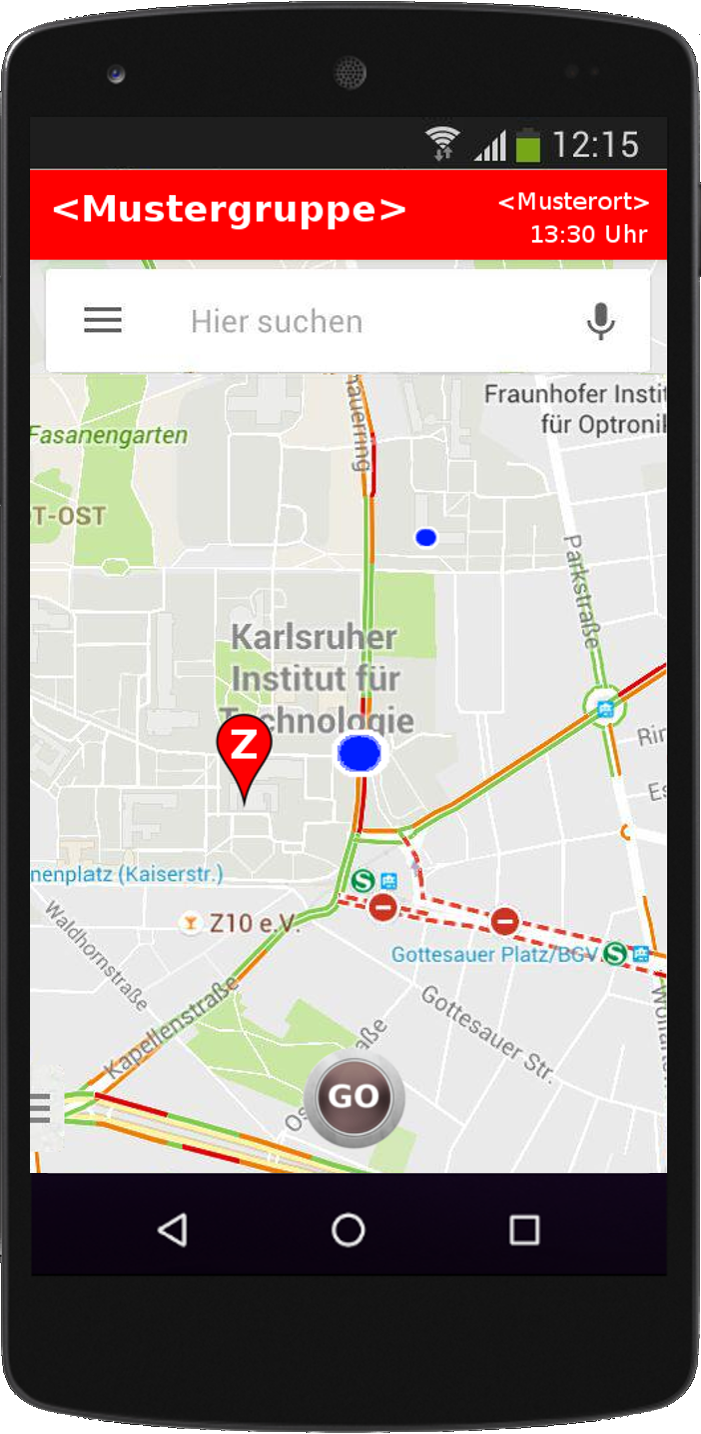
\includegraphics[scale =0.2]{resources/images/handy/map_go.png}
%\end{center}
\end{wrapfigure}
\textbf{Beschreibung:}\\
Kartenansicht der Gruppe wenn der "Go"-Button schon gedrückt ist. Allen GM wird in dieser Ansicht nicht nur die Karte angezeigt, sondern auch der Zielort und die Uhrzeit des nächsten festgelegten Treffpunktes, außerdem noch auf der Karte der Zielort durch eine Stecknadel beschriftet mit "Z" und die Standorte der anderen GMer durch blaue Kreise. Je größer ein Kreis, desto mehr GM befinden sich an dem gleichen Standort.\\
\textbf{Elemente:}\\
"Gruppenname"-Button um zu den Gruppendetails zu gelangen.\\
"Zielort - Uhrzeit"-Ansicht zur Orientierung wann und wo das nächste Treffen festgelegt ist, bzw. "Zielort - Uhrzeit"-Button bei der Ansicht des GA um ein neues Treffen zu erstellen.\\
"Hier suchen"-Textfeld um einen Ort auf der Karte zu suchen.\\
Lupen-Button um die Suche zu starten.\\
Handle links unten in der Ecke um die Gruppenansicht wieder herauszuziehen.\\
Deaktivierter "Go"-Button um das Versenden des eigenen Standortes zu stoppen.\\
Blaue Kreise zur Orientierung, wo sich die anderen GM befinden.\\
\textbf{Verwendung:}\\
Durch einmaliges Tippen auf den "Gruppenname"-Button wird das GM weiter geleitet zu der Ansicht "Gruppendeteils".\\
Durch einmaliges Tippen auf den "Zielort - Uhrzeit"-Button wird der GA weiter geleitet zu der Option "Treffen erstellen".\\
Durch einmaliges Tippen auf das Textfeld "Hier suchen" wird die Bildschirmtastatur aktiviert und das GM kann seinen gewählten Zielort eingeben.\\
Durch einmaliges Tippen auf den Lupen-Button wird eine Suche nach dem gewählten Zielort gestartet und die Ergebnisse dem GM angezeigt.\\
Durch Streichen von links nach rechts über den Hanlde-Button kann das GMG die Gruppenansicht wieder herausziehen.\\
Durch einmaliges Tippen auf den "Go"-Button wird dieser deaktiviert und das Senden des Standortes des GM wird gestoppt. Außerdem kann das GM dann nicht mehr die Standorte der anderen GM sehen (Ansicht: "Kartenansicht der Gruppe").
\newpage


\begin{wrapfigure} {L}{0.35\textwidth}
	\caption{Benutzername ändern (Wunschkriterium)}
	%\begin{center}
		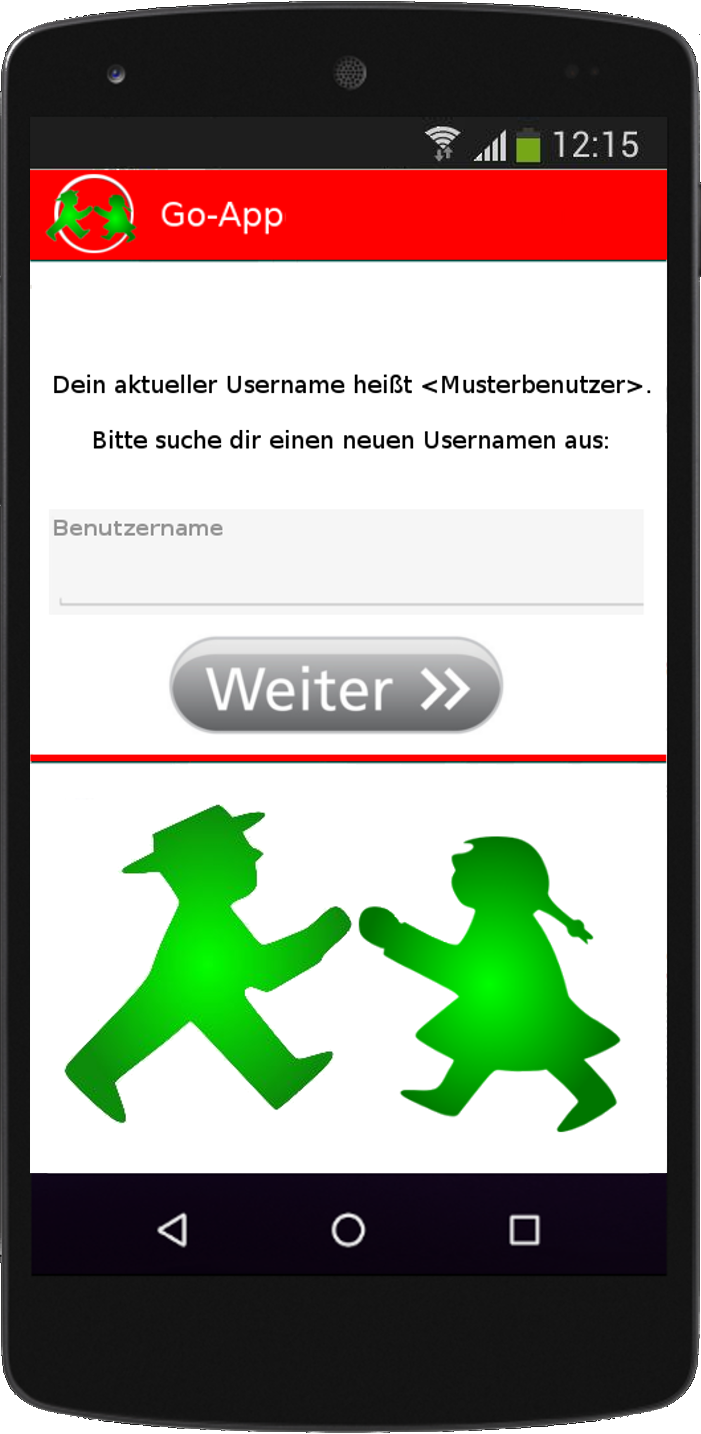
\includegraphics[scale =0.2]{resources/images/handy/username_aendern.png}
	%\end{center}
\end{wrapfigure}

\textbf{Beschreibung:}\\
Option zum ändern des BNs(Benutzernamen), Information über den aktuellen BN und Aufforderung an den Benutzer sich einen neuen BN zu wählen.\\
\textbf{Elemente:}\\
BN zur Orientierung, mit welchem Namen der Benutzer registriert ist.\\
Textfeld "Benutzername" zum Einfügen des BNs.\\
"Weiter"-Button um diesen zu bestätigen.\\
\textbf{Verwendung:}\\
Durch einmaliges Tippen auf das Textfeld "Benutzername" wird die Bildschirmtastatur aktiviert und der Benutzer kann seinen gewählten BN eingeben.\\
Durch einmaliges Tippen auf den "Weiter"-Button wird dieser BN bestätigt und der Benutzer wird weitergeleitet zu der Gruppenübersicht.